
\label{chapter:unit_tests}

In addition to the \maestro\ science problems, which use the full
capabilities of \maestro, there are a number of unit tests that
exercise only specific components of the \maestro\ solvers.  These
tests have their own drivers (a custom \code{varden.f90}) that
initialize only the data needed for the specific test and call
specific \maestro\ routines directly.


\section {\tt test\_advect}

  This test initializes a Gaussian density field (no other scalar
  quantities are used) and a uniform velocity field in any one of the
  coordinate directions.  The Gaussian profile is advected through the
  period domain exactly once and the error in the density profile (L2
  norm) is computed.  The driver for this problem does this for every
  dimension twice (once with a positive velocity and once with a
  negative velocity), and loops over all advection methods
  (\runparam{ppm\_type} {\tt = 0,1,2} and \runparam{bds\_type} {\tt = 1}).  After
  all coordinate directions are tested, the norms are compared to
  ensure that the error does not show any directional bias.

  Note: the BDS advection method does not guarantee that the error be
  independent of the advection direction---small differences can
  arise.  What's happening here is that within each cell BDS is trying
  to define a tri-linear profile for rho subject to the constrants in
  the BDS paper~\cite{bds3d} (constraints 1 and 2 on p.\ 2044 after eq. 3.4).  We
  do not solve the L2 minimization problem exactly so we iterate up to
  3 times using a simple heuristic algorithm designed to work toward
  the constraint.  The iteration will give different results depending
  on orientation since we work through the corners in arbitrary order.

\begin{figure}[t] 
\centering
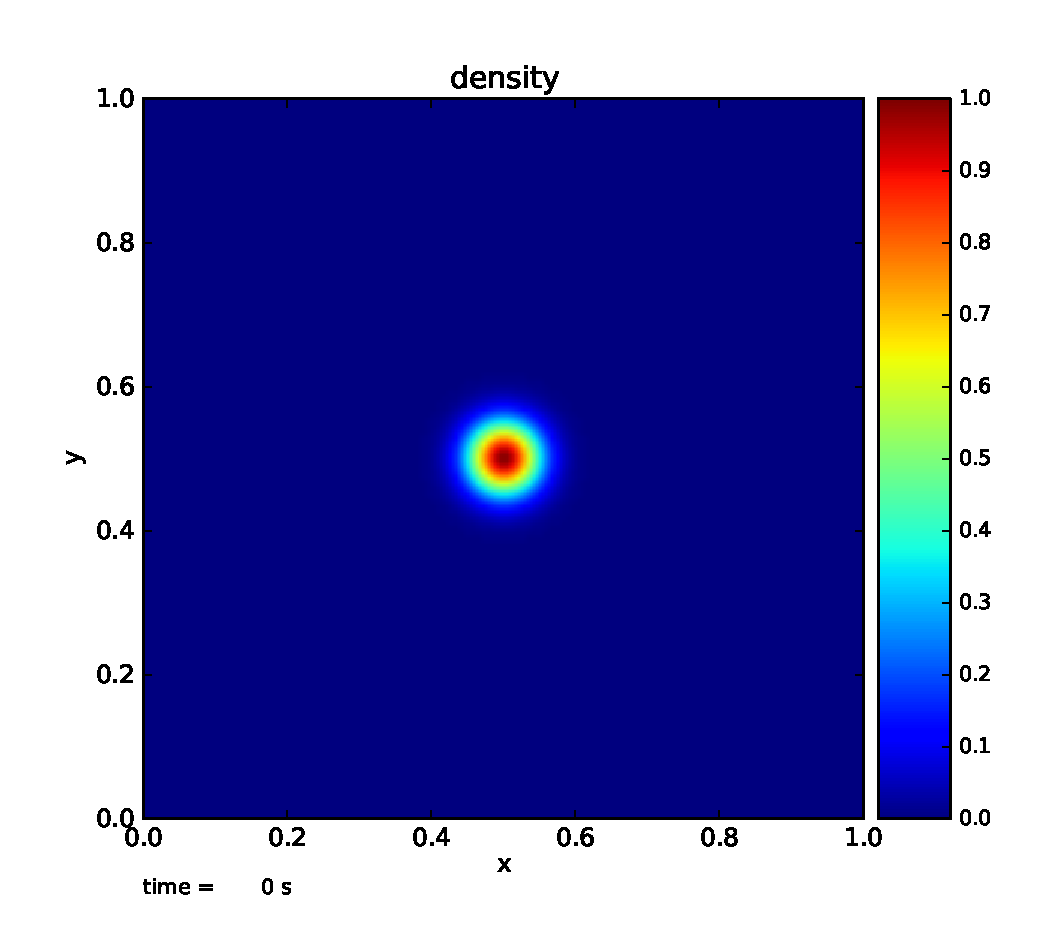
\includegraphics[height=1.9in]{\unitfigpath/dens_2d_orig_density}
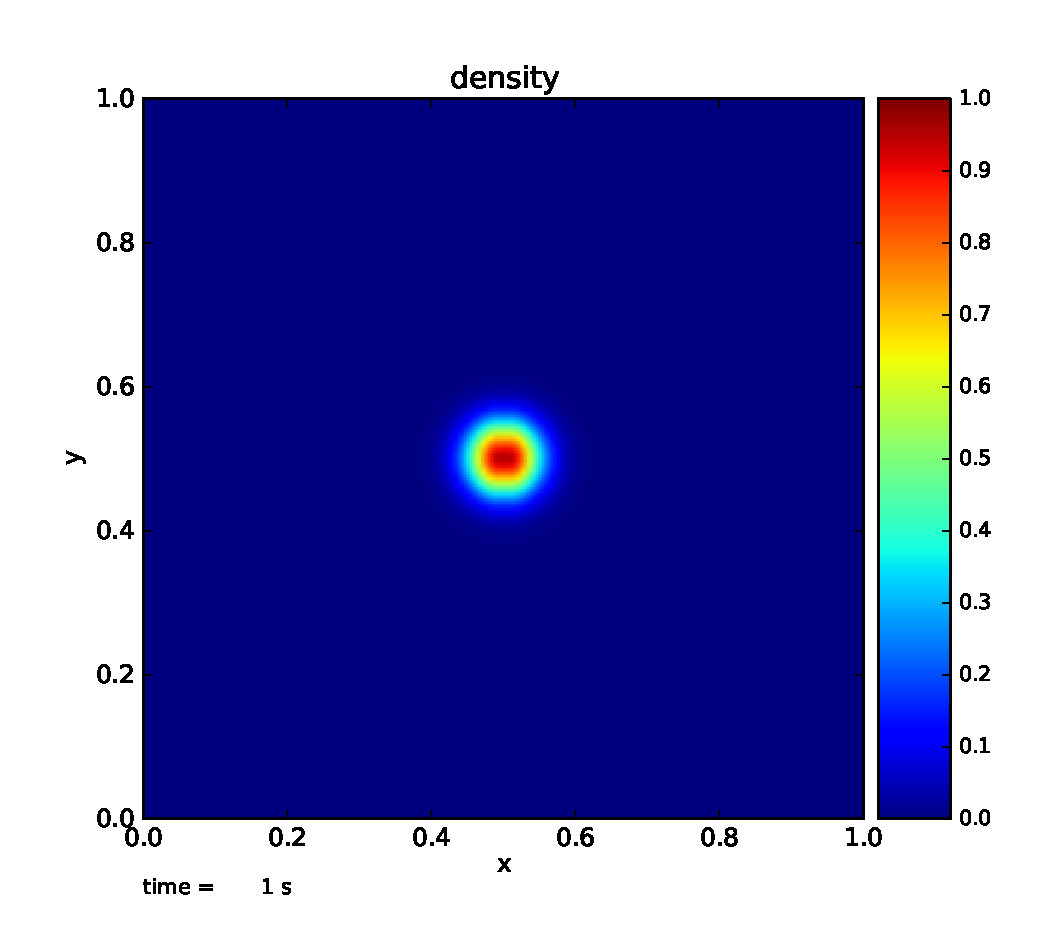
\includegraphics[height=1.9in]{\unitfigpath/dens_2d_ppm1_xp_final_density}
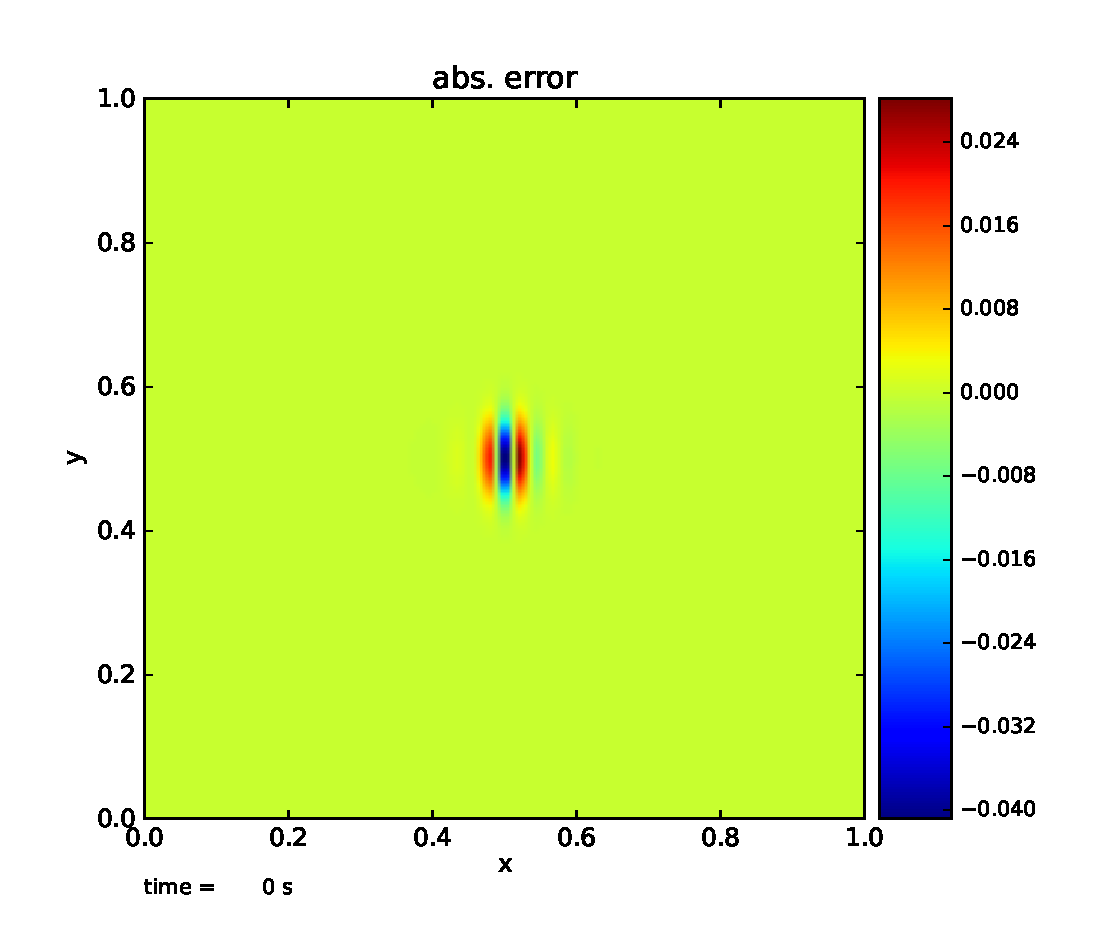
\includegraphics[height=1.9in]{\unitfigpath/dens_2d_ppm1_xp_final_abserror} 
%
\caption[Results of the {\tt test\_advect} unit test]{\label{fig:unit:advtest}
  Initial Gaussian density profile (left); density profile after
  advecting to the right for one period (center); absolute error
  between the final and initial density fields, showing the error in
  the advection scheme (right).}
\end{figure}


\section {\tt test\_average} 

  This test initializes a 1D radial base state quantity with a
  Gaussian distribution, maps it into the 3D domain (assuming a
  spherical geometry) using the routines provided by
  the \code{fill\_3d\_module} module, and then calls \code{average} to
  put it back onto a 1D radial array.  This way we test the accuracy
  of our procedure to map between the 1D radial and 3D Cartesian
  states.  The output from this test was described in detail
  in \cite{multilevel}.


\section {\tt test\_basestate} 

  This test initializes the base state to contain a hydrostatic
  model and then evolves the state with heating to watch the 
  hydrostatic adjustment of the atmosphere.  In particular,
  the base state velocity, $w_0$, is computed in response to 
  the heating and this is used to advect the base state density
  and compute the new pressure, $p_0$.  An early version of 
  this routine was used for the plane-parallel expansion test
  in \cite{lowMach2}.  This version of the test was also shown
  for a spherical, self-gravitating star in \cite{multilevel}.

  
\section {\tt test\_diffusion}

  This test initializes a Gaussian temperature profile and calls
  the thermal diffusion routines in \maestro\ to evolve the state 
  considering only diffusion.  The driver estimates a timestep
  based on the explicit thermal diffusion timescale and loops
  over calls to the thermal diffusion solver.  A Gaussian remains
  Gaussian when diffusing, so an explicit error can be computed
  by comparing to the analytic solution.  This test is 
  described in \cite{xrb}.


\section {\tt test\_eos}

  This test sets up a 3-d cube with $\rho$ varying on one axis, $T$ on
  another, and the composition on the third.  The EOS is then called
  in every zone, doing $(\rho, T) \rightarrow  p, h, s, e$  and stores those
  quantities.  Then it does each of the different EOS types to recover
  either $T$ or $\rho$ (depending on the type), and stores the new $T$ (or
  $\rho$) and the relative error with the original value.  A plotfile is
  stored holding the results and errors.  This allows us to determine
  whether the EOS inversion routines are working right.


\section {\tt test\_particles}

  This test exercises the particle advection routine.  A simple
  circular velocity field, with the magnitude increasing with radius
  from the center is initialized.  A number of particles are then
  initialized at various radii from the center and they are advected
  for one period.  The particle paths should be perfect circles, and
  the final particle position should overlap with the initial
  position.

  Particle data is stored separately from the fluid data.  Instead
  of being part of the plotfiles, the particle data is outputted
  each timestep into files named {\tt timestamp\_*}, where 
  the number indicates which processor did the writing.  These
  particle files can be processed and the particle data plotted
  using the python routines in {\tt data\_processing/python/}.

  The output from this test can be visualized with the script {\tt
  plot.py} in the test directory.  The output shows the particle
  paths (see figure~\ref{fig:unit:particles}).

\begin{figure}[t] 
\centering
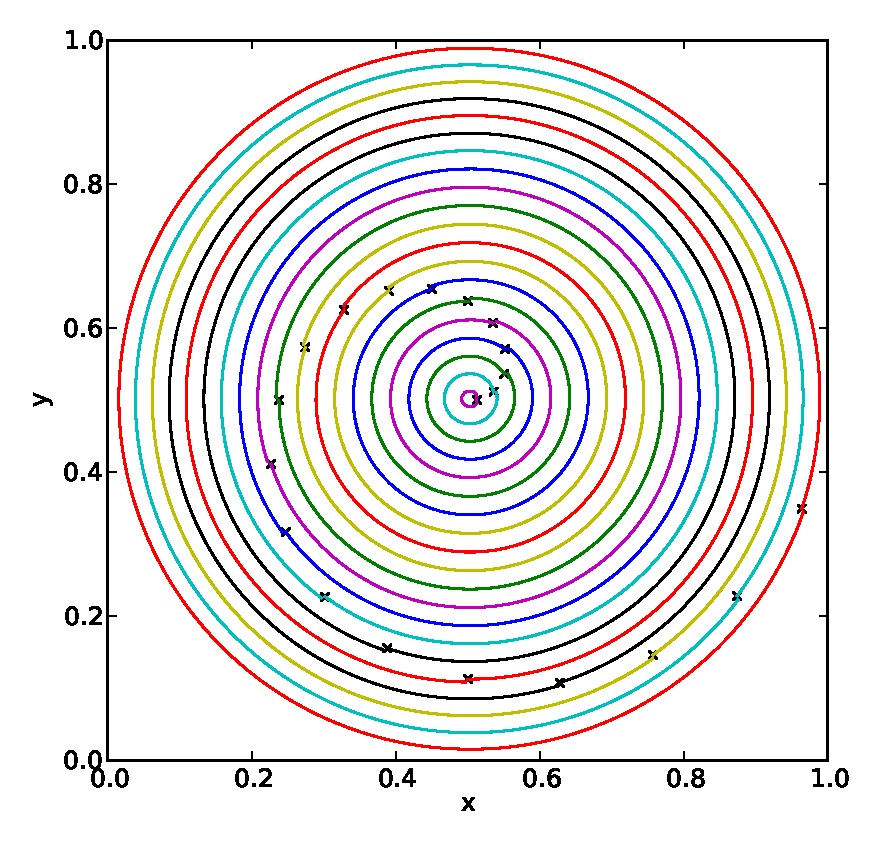
\includegraphics[width=4in]{\unitfigpath/particle_paths} 
%
\caption[Particle paths for the {\tt test\_particles} problem]{\label{fig:unit:particles}
  Particle paths for the {\tt test\_particles} problem.  The initial
  position of the particles is marked with an $\times$.}
\end{figure}


\section {\tt test\_projection}

  This tests the projection routines in 2- and 3-d---either the hgprojection
  ({\tt project\_type = 1}) or the MAC projection ({\tt project\_type =
  2}).  A divergence-free velocity field is initialized and then
  ``polluted'' by adding the gradient of a scalar.  The form of the
  scalar differs depending on the boundary conditions (wall and
  periodic are supported currently).  Finally, the hgproject routine
  is called to recover the initial divergence-free field.
  Figure~\ref{fig:unit:projtest} shows the initial field, polluted
  field, and result of the projection for the hgproject case.

\begin{figure}[t] 
\centering
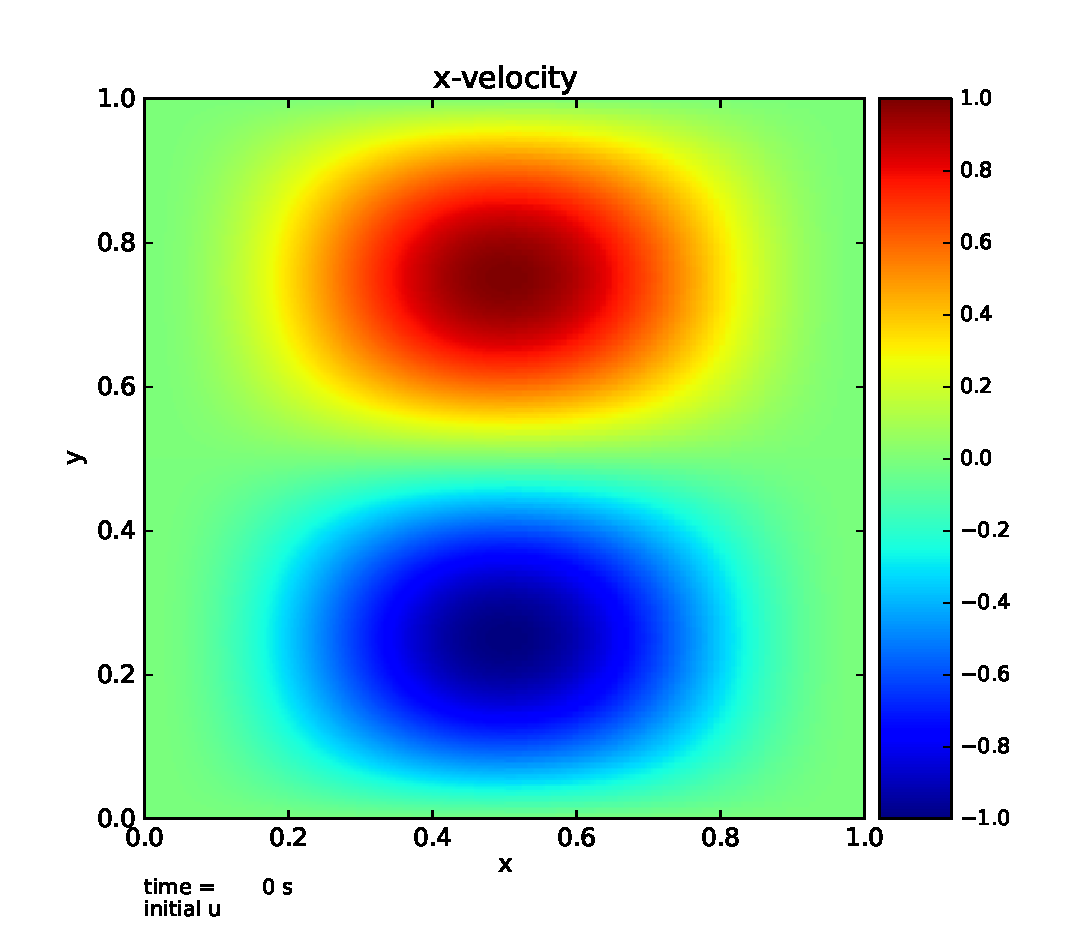
\includegraphics[height=1.9in]{\unitfigpath/wall_u_init_x-velocity} 
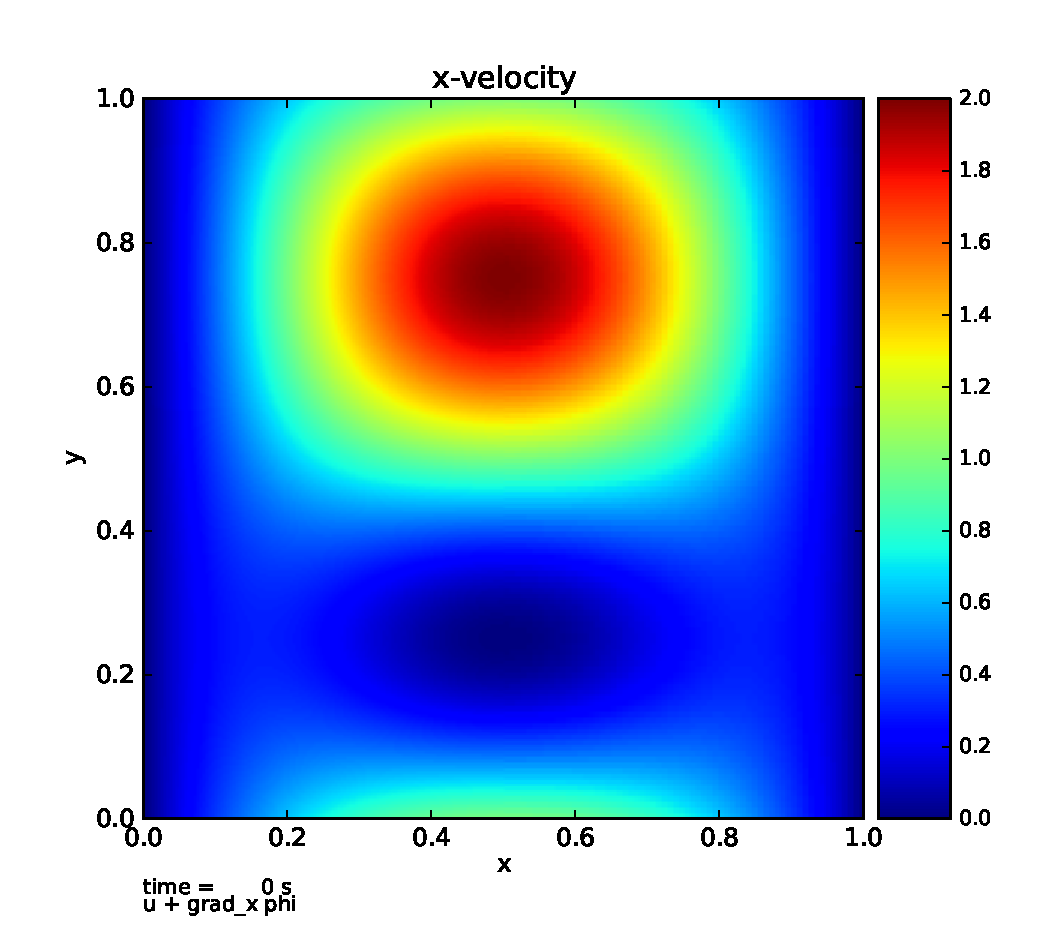
\includegraphics[height=1.9in]{\unitfigpath/wall_u_plus_grad_phi_x-velocity} 
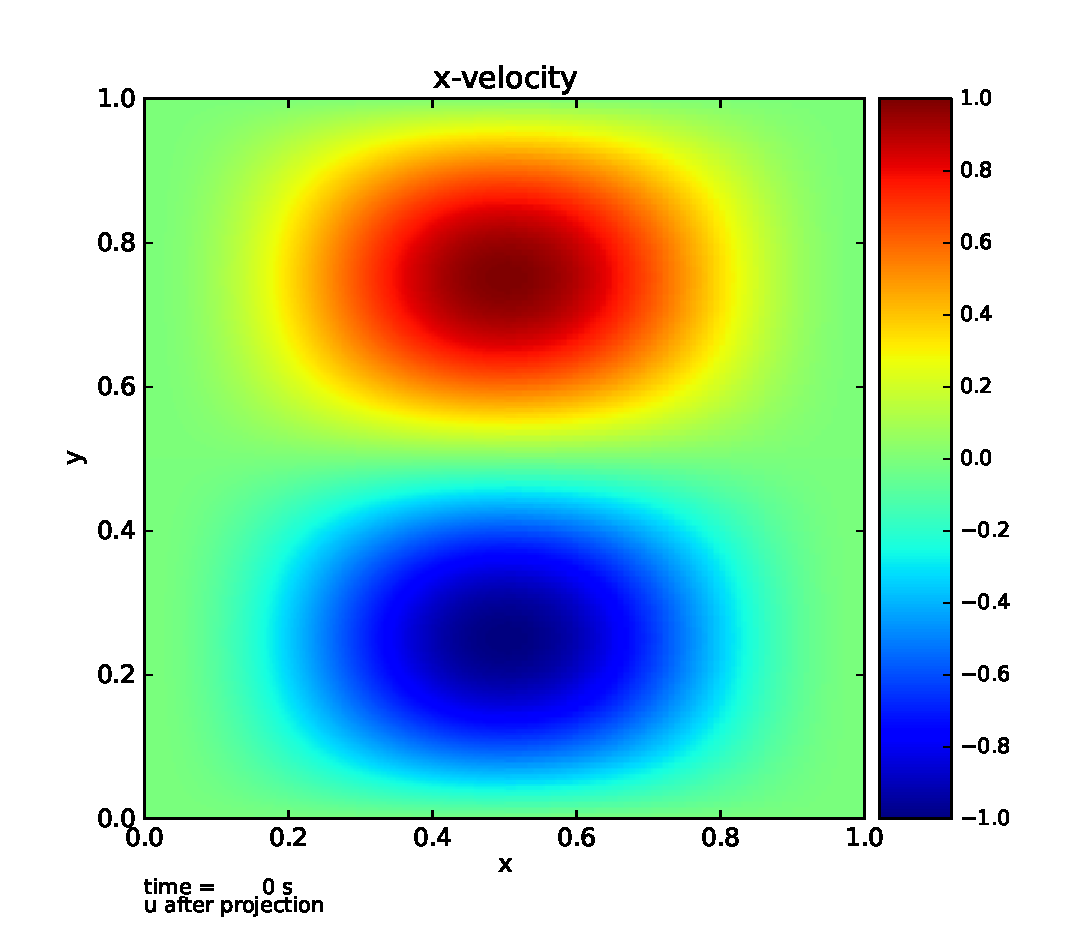
\includegraphics[height=1.9in]{\unitfigpath/wall_u_new_x-velocity} 
%
\caption[Results of the 2-d {\tt test\_projection} unit test]{\label{fig:unit:projtest}
  Initial divergence free velocity field (x-component; left); Velocity
  field plus gradient of a scalar (x-component; center); and resulting
  velocity after projecting out the non-divergence free portion
  (x-component; right).  This is with slipwall boundary conditions on
  all sides, a 2-level grid with the left half refined and right half
  coarse, and the hgprojection tested.}
\end{figure}


\begin{figure}
\centering
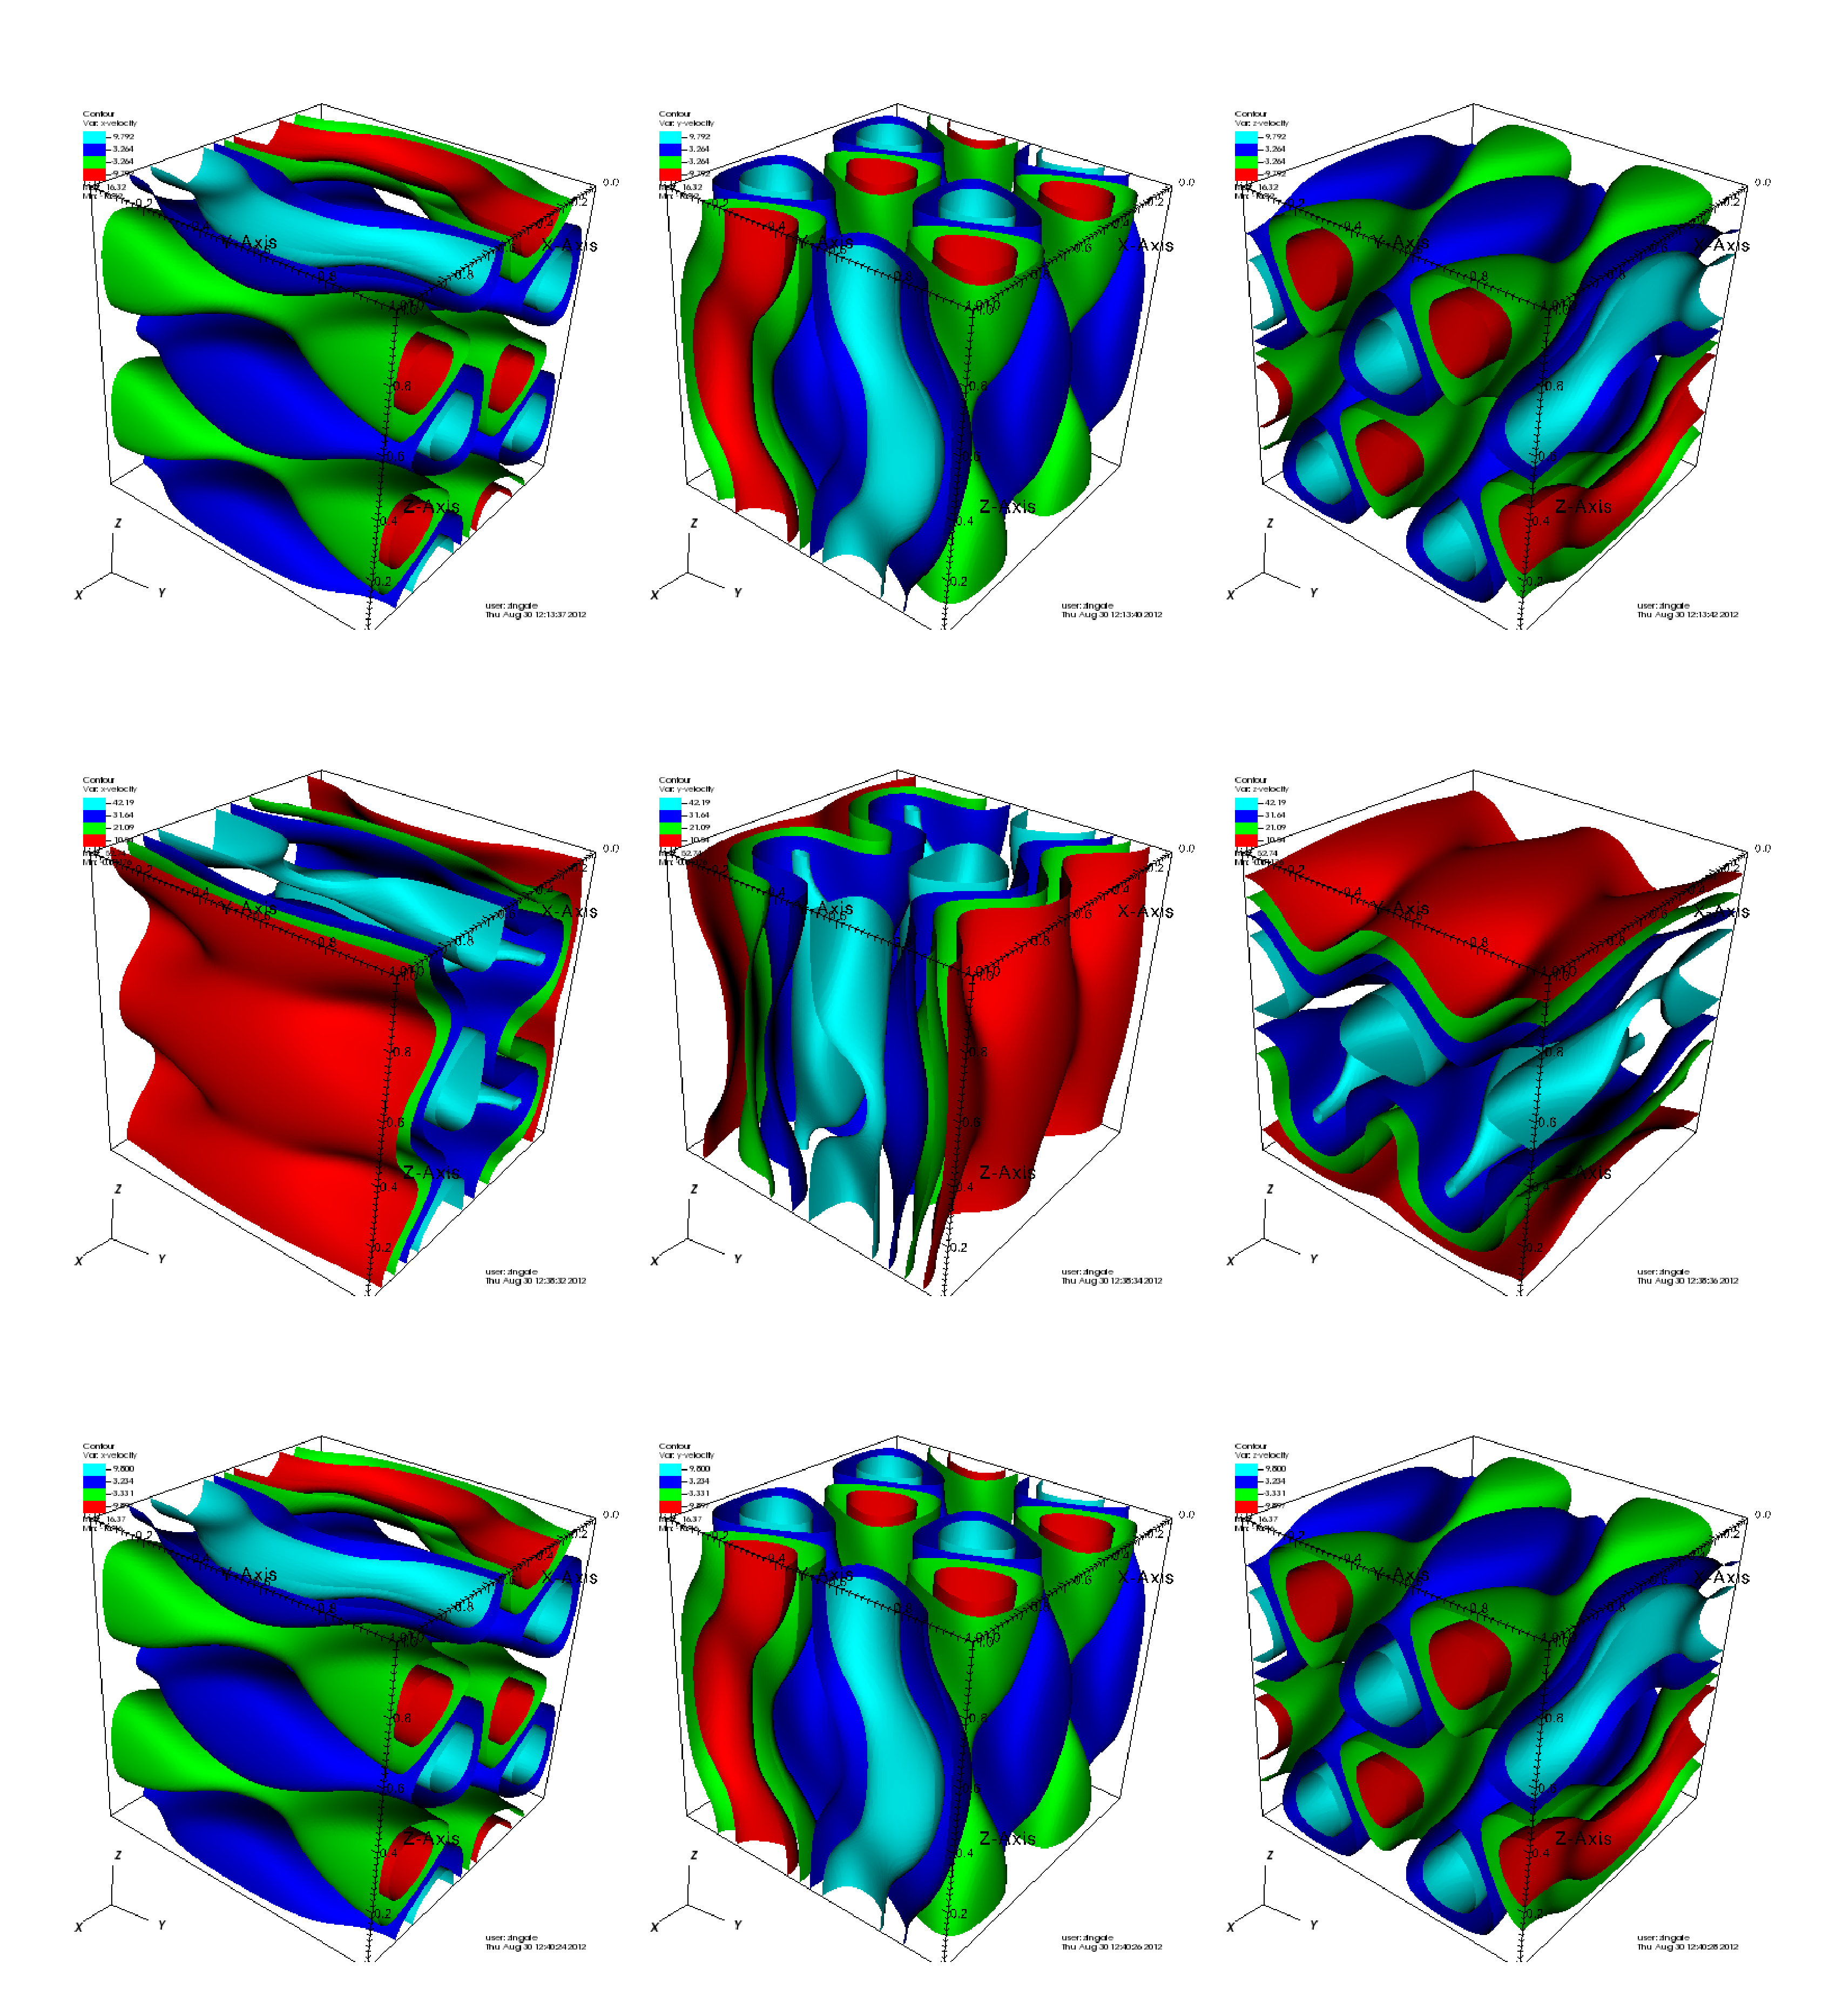
\includegraphics[height=8in]{\unitfigpath/test_project_3d}
%
\caption[Results of the 3-d {\tt test\_projection} unit test]{\label{fig:unit:projtest3d}
  Projection test in 3-d showing the x-velocity (left), y-velocity
  (middle), and z-velocity (right) initially (top row), after the
  gradient of a scalar is added (center row), and the resulting
  velocity after the projection.  This is with slipwall boundary conditions
  on all sides, a 2-level grid with an octant refined, and the hgprojection.}
\end{figure}

\section{\tt test\_react}

  This simply tests the reaction network by calling
  the \maestro\ \code{react\_state} routine directly.  The network is
  selected in the {\tt GNUmakefile} by setting the {\tt NETWORK\_DIR}
  variable.  A 3d cube is setup with density varying on one axis,
  temperature varying on another, and the composition varying on the
  third.  The density and temperature ranges are set in the inputs
  file.  The composition is read in via an input file.

  A good use of this test is to test whether a burner is threadsafe.
  This is accomplished by compiling with OpenMP (setting {\tt OMP=t})
  and the running with 1 thread and multiple threads (this can be done
  by setting the environment variable {\tt OMP\_NUM\_THREADS} to the 
  desired number of threads).  Since each zone is independent of the
  others, the results should be identical regardless of the number
  of threads.  This can be confirmed using the {\tt fcompare} tool
  in {\tt AmrPostprocessing}.


